\documentclass[tikz,border=10pt]{standalone}
\usetikzlibrary{arrows.meta, decorations.markings}

\tikzset{
    fermion/.style={draw=red, thick, ->},
    bsm/.style={draw=gray, thick, ->},
    sm/.style={draw=black, thick, ->},
    decoration={
        markings,
        mark=at position 0.5 with {\arrow[thick]{>}}
    }
}

\begin{document}
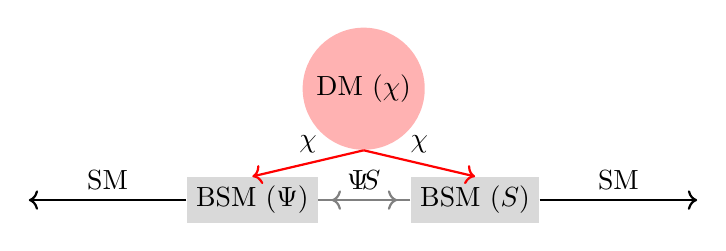
\begin{tikzpicture}[node distance=2cm]

\node (DM) [circle, fill=red!30] at (0,0) {DM (\(\chi\))};
\node (BSM1) [rectangle, fill=gray!30, below left of=DM] {BSM (\(\Psi\))};
\node (BSM2) [rectangle, fill=gray!30, below right of=DM] {BSM (\(S\))};

% Fermionic DM lines
\draw[fermion] (DM.south) -- node[midway, above] {$\chi$} (BSM1.north);
\draw[fermion] (DM.south) -- node[midway, above] {$\chi$} (BSM2.north);

% BSM particle lines
\draw[bsm] (BSM1.east) -- node[midway, above] {$\Psi$} ++(1,0);
\draw[bsm] (BSM2.west) -- node[midway, above] {$S$} ++(-1,0);

% SM particle line
\draw[sm] (BSM1.west) -- node[midway, above] {SM} ++(-2,0);
\draw[sm] (BSM2.east) -- node[midway, above] {SM} ++(2,0);

\end{tikzpicture}
\end{document}